% --------------------------------------------------------------
% This is all preamble stuff that you don't have to worry about.
% Head down to where it says "Start here"
% --------------------------------------------------------------
 
\documentclass[12pt]{article}
 
\usepackage[margin=1in]{geometry} 
\usepackage{amsmath,amsthm,amssymb,listings,xcolor,graphicx}
 
\DeclareMathOperator{\sinc}{sinc}

\newcommand{\N}{\mathbb{N}}
\newcommand{\Z}{\mathbb{Z}}
 
\newenvironment{theorem}[2][Theorem]{\begin{trivlist}
\item[\hskip \labelsep {\bfseries #1}\hskip \labelsep {\bfseries #2.}]}{\end{trivlist}}
\newenvironment{lemma}[2][Lemma]{\begin{trivlist}
\item[\hskip \labelsep {\bfseries #1}\hskip \labelsep {\bfseries #2.}]}{\end{trivlist}}
\newenvironment{exercise}[2][Exercise]{\begin{trivlist}
\item[\hskip \labelsep {\bfseries #1}\hskip \labelsep {\bfseries #2.}]}{\end{trivlist}}
\newenvironment{problem}[2][Problem]{\begin{trivlist}
\item[\hskip \labelsep {\bfseries #1}\hskip \labelsep {\bfseries #2.}]}{\end{trivlist}}
\newenvironment{question}[2][Question]{\begin{trivlist}
\item[\hskip \labelsep {\bfseries #1}\hskip \labelsep {\bfseries #2.}]}{\end{trivlist}}
\newenvironment{corollary}[2][Corollary]{\begin{trivlist}
\item[\hskip \labelsep {\bfseries #1}\hskip \labelsep {\bfseries #2.}]}{\end{trivlist}}

\newenvironment{solution}{\begin{proof}[Solution]}{\end{proof}}

\definecolor{codegreen}{rgb}{0,0.6,0}
\definecolor{codegray}{rgb}{0.5,0.5,0.5}
\definecolor{codepurple}{rgb}{0.58,0,0.82}
\definecolor{backcolour}{rgb}{0.97,0.97,0.97}
\lstdefinestyle{pystyle}{
    backgroundcolor=\color{backcolour},   
    commentstyle=\color{codegreen},
    keywordstyle=\color{magenta},
    numberstyle=\tiny\color{codegray},
    stringstyle=\color{codepurple},
    basicstyle=\ttfamily\small,
    breakatwhitespace=false,         
    breaklines=true,                 
    captionpos=b,                    
    keepspaces=true,                 
    numbers=left,                    
    numbersep=5pt,                  
    showspaces=false,                
    showstringspaces=false,
    showtabs=false,                  
    tabsize=2
}
\lstset{style=pystyle}

\graphicspath{{./figures}}
 
\begin{document}
 
\title{Homework 1: Sampling And Aliasing}
\author{Matthew Luyten\\ %replace with your name
ECE6250}

\maketitle

\begin{enumerate} 
\item[] 1.1 Summary and Context of Sampling

This week we covered sampling and aliasing, which is foundational in modern signal processing. 
Using computers, ADCs, and DACs, engineers have significantly more flexibility processing discrete 
sampled signals than their continuous time counterparts. Due to this versatility, the vast majority of 
continuous time signals we process and analyze are discretized through sampling, so modern engineers 
must have a strong understanding of it. The nyquist-shannon sampling theorem is the most 
foundational part of this understanding, and its simplest rule, the Nyquist criterion, must be 
considered in any sampling application. Violating the Nyquist criterion results in the other 
foundational concept of sampling: aliasing.

In any sampling application, the first question must be: “Can I satisfy the Nyquist Criterion?". If not,
most likely, you will not be able to capture the signal you desire. In specific applications, like the
one mentioned in class by Dr. Anderson, aliasing can actually be powerful tool. However, this tool, and 
others like it, require a stong fundamental understanding of sampling.

It may be a bit reductive, but the D in DSP stands for Digital, which implies we work in the discrete domain.
However, we live in the continuous domain. Sampling, thus, underpins everything we do in DSP.

\newpage

\item[] 1.5a

\begin{figure}[h]
    \caption{$h[n]=\sinc(\frac{\pi n}{M})$, $n\in[-20,20]$, $M=7$}
    \centering
    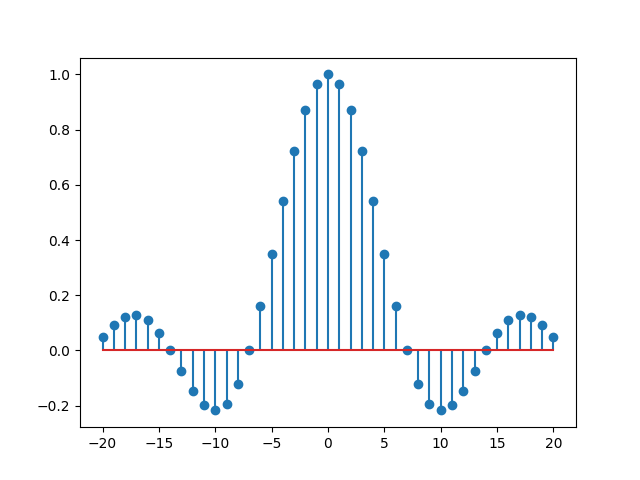
\includegraphics[scale=0.6]{1-5a.png}
\end{figure}

\noindent Python Code for Figure 1:

\begin{lstlisting}[language=Python]
import numpy as np
import matplotlib.pyplot as plt

if __name__ == "__main__":
    n = np.linspace(-20, 20, 41)
    M = 7
    h_n = np.sinc(n / M)

    plt.stem(n, h_n)
    plt.show()
\end{lstlisting}
\newpage

\item[] 1.5b

\begin{figure}[h]
    \caption{
        $x(t)=(\frac{1}{2B+1})(\frac{\cos(2\pi Bt)-\cos(2\pi(B+1)t)}{1-\cos(2\pi t)})$, 
        $t\in[-\frac{1}{2}, \frac{1}{2}]$, $B=9$
        }
    \centering
    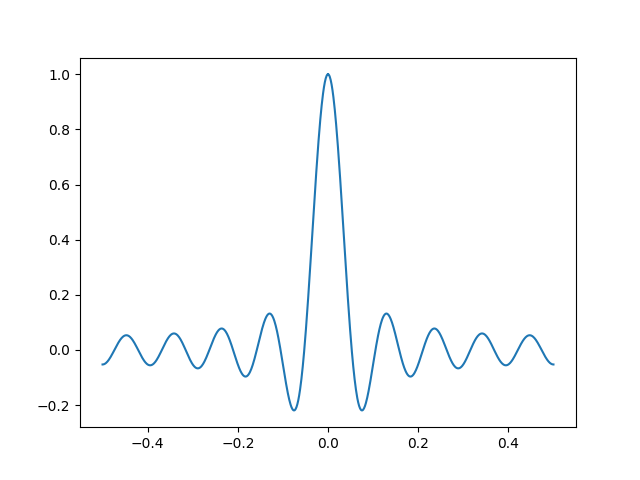
\includegraphics[scale=0.6]{1-5b.png}
\end{figure}

\noindent Python Code for Figure 2:

\begin{lstlisting}[language=Python]
import numpy as np
import matplotlib.pyplot as plt

if __name__ == "__main__":
    t = np.linspace(-0.5, 0.5, 1001)
    B = 9
    x_t = (np.cos(2*np.pi*B*t)-np.cos(2*np.pi*(B+1)*t))/((2*B+1)*(1.-np.cos(2*np.pi*t)))

    plt.plot(t, x_t)
    plt.show()
\end{lstlisting}
\newpage

\item[]  1.5c

\begin{figure}[h]
    \caption{
        $x(t)=(\frac{1}{2B+1})(\frac{\cos(\frac{2\pi Bn}{N})-\cos(\frac{2\pi(B+1)n}{N}))}{1-\cos(\frac{2\pi n}{N})})$, 
        $t\in[-\frac{1}{2}, \frac{1}{2}]$, $B=9$
        }
    \centering
    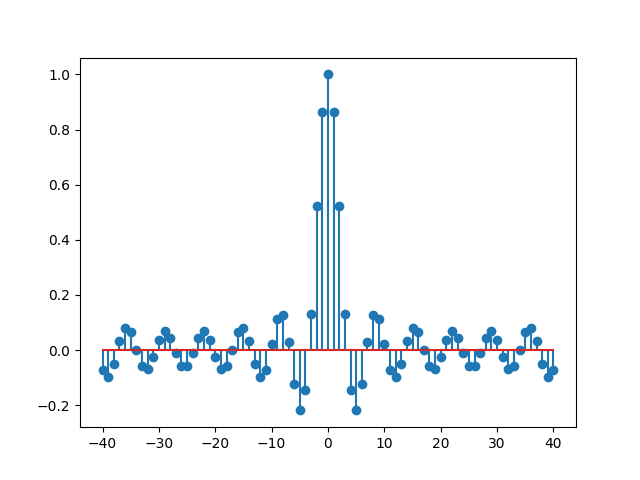
\includegraphics[scale=0.6]{1-5c.png}
\end{figure}

\noindent Python Code for Figure 3:

\begin{lstlisting}[language=Python]
import numpy as np
import matplotlib.pyplot as plt

if __name__ == "__main__":
    n = np.linspace(-40, 40, 81)
    n[40] = 1e-6 # if this is 0, divide by 0 error happens. This gets us close
    N = 51
    B = 7
    x_n = (np.cos(2*np.pi*B*n/N)-np.cos(2*np.pi*(B+1)*n/N))/((2*B+1)*(1.-np.cos(2*np.pi*n/N)))

    plt.stem(n, x_n)
    plt.show()
\end{lstlisting}
\newpage

\end{enumerate}
 
\end{document}
